% !TeX program = xelatex
\documentclass[tikz, border=2pt]{standalone}
\usepackage{ctex}
\usepackage{tikz}
\usetikzlibrary{shadows, positioning, arrows.meta, decorations.pathmorphing, fit, backgrounds, calc}
\begin{document}
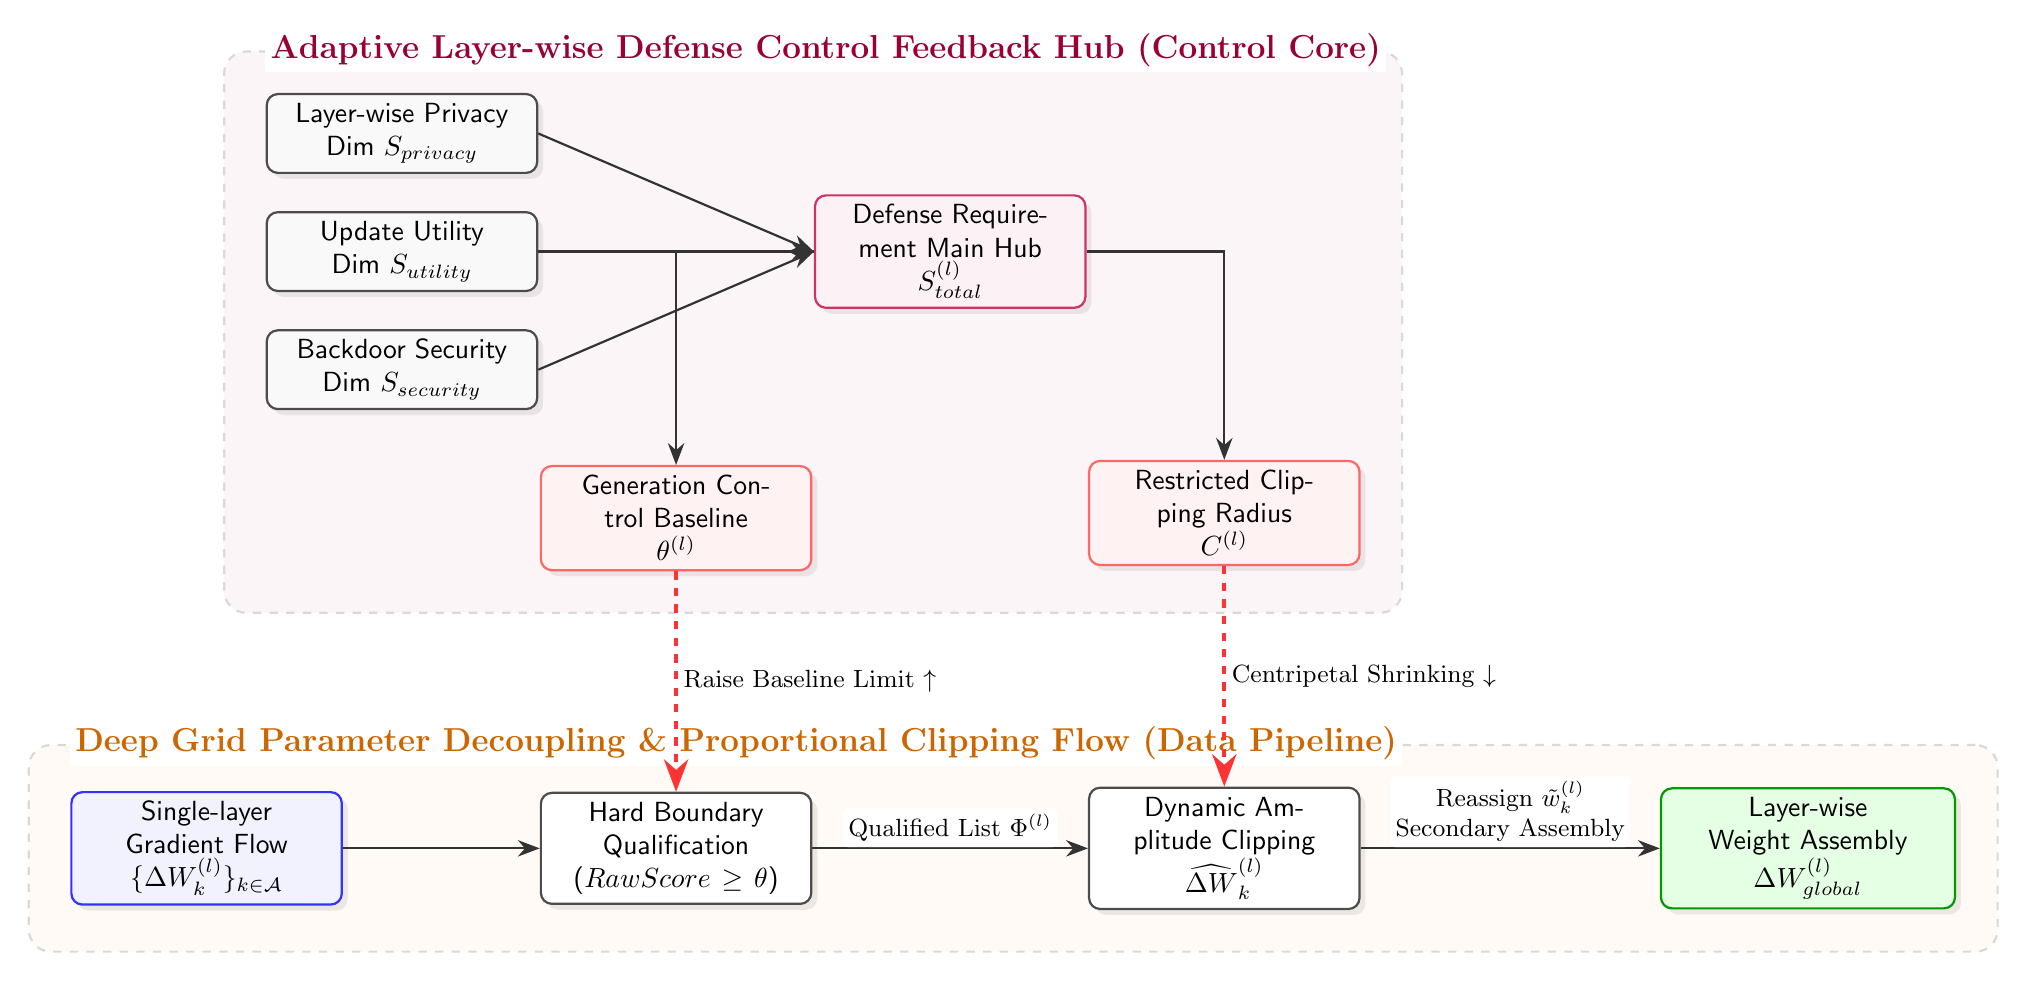
\begin{tikzpicture}[
        font=\sffamily,
        >=Stealth,
        % Styles
        phase_bg/.style={draw=gray!30, fill=#1, rounded corners=8pt, inner sep=15pt, dashed, thick},
        block/.style={draw=black!70, fill=white, rounded corners=4pt, text width=3.2cm, align=center, minimum height=1.3cm, thick, drop shadow={opacity=0.15}},
        small_block/.style={block, minimum height=0.8cm, text width=3.2cm, fill=white!95!gray},
        highlight_block/.style={block, fill=red!5, draw=red!60, thick},
        final_block/.style={block, fill=green!10, draw=green!60!black, thick, text width=3.5cm},
        arrow/.style={-{Stealth[scale=1.2]}, thick, draw=black!80},
        lbl/.style={fill=white, inner sep=2pt, font=\small, rounded corners=2pt}
    ]

    % Core Data Nodes (Bottom Row)
    \node[block] (survivors) {Hard Boundary Qualification\\($RawScore \ge \theta$)};
    \node[block, left=2.5cm of survivors, fill=blue!5, draw=blue!80] (data_in) {Single-layer Gradient Flow\\$\{\Delta W_{k}^{(l)}\}_{k \in \mathcal{A}}$};
    \node[block, right=3.5cm of survivors] (clipped) {Dynamic Amplitude Clipping\\$\widehat{\Delta W}_{k}^{(l)}$};
    \node[final_block, right=3.8cm of clipped] (agg) {Layer-wise Weight Assembly\\$\Delta W_{global}^{(l)}$};
    
    \draw[arrow] (data_in) -- (survivors);
    \draw[arrow] (survivors) -- node[lbl, above] {Qualified List $\Phi^{(l)}$} (clipped);
    \draw[arrow] (clipped) -- node[lbl, above, align=center] {Reassign $\tilde{w}_k^{(l)}$\\Secondary Assembly} (agg);

    % Control Nodes (Intermediate)
    \node[highlight_block, above=2.8cm of survivors] (theta) {Generation Control Baseline\\$\theta^{(l)}$};
    \node[highlight_block, above=2.8cm of clipped] (clip) {Restricted Clipping Radius\\$C^{(l)}$};

    \draw[arrow, dashed, draw=red!80, line width=1.5pt] (theta) -- node[lbl, right] {Raise Baseline Limit $\uparrow$} (survivors);
    \draw[arrow, dashed, draw=red!80, line width=1.5pt] (clip) -- node[lbl, right] {Centripetal Shrinking $\downarrow$} (clipped);

    % Control Nodes (Top S_total)
    \path (theta) -- node[pos=0.5] (mid_tc) {} (clip);
    \node[block, fill=purple!5, draw=purple!80, above=2.5cm of mid_tc] (stotal) {Defense Requirement Main Hub\\$S_{total}^{(l)}$};
    
    \draw[arrow] (stotal) -| (theta);
    \draw[arrow] (stotal) -| (clip);

    % Sensors
    \node[small_block, left=3.5cm of stotal, yshift=1.5cm] (sp) {Layer-wise Privacy Dim $S_{privacy}$};
    \node[small_block, left=3.5cm of stotal, yshift=0cm] (su) {Update Utility Dim $S_{utility}$};
    \node[small_block, left=3.5cm of stotal, yshift=-1.5cm] (ss) {Backdoor Security Dim $S_{security}$};

    \draw[arrow] (sp.east) -- (stotal.west);
    \draw[arrow] (su.east) -- (stotal.west);
    \draw[arrow] (ss.east) -- (stotal.west);
    
    % Grouping Backgrounds
    \begin{scope}[on background layer]
        \node[phase_bg=purple!4, fit=(sp) (ss) (stotal) (theta) (clip)] (bgControl) {};
        \node[font=\bfseries\large, text=purple!80!black, fill=white, inner sep=2pt] at (bgControl.north west) [anchor=south west, xshift=15pt, yshift=-8pt] {Adaptive Layer-wise Defense Control Feedback Hub (Control Core)};
        
        \node[phase_bg=orange!4, fit=(data_in) (survivors) (clipped) (agg)] (bgData) {};
        \node[font=\bfseries\large, text=orange!80!black, fill=white, inner sep=2pt] at (bgData.north west) [anchor=south west, xshift=15pt, yshift=-8pt] {Deep Grid Parameter Decoupling \& Proportional Clipping Flow (Data Pipeline)};
    \end{scope}

    \end{tikzpicture}
\end{document}
